--- /home/jesse/Analysis/FemtoAnalysis/LamKPublication/CERN/Comments2/LamKPublication_v3A.tex
+++ /home/jesse/Analysis/FemtoAnalysis/LamKPublication/CERN/Comments2/LamKPublication_v3B.tex
@@ -2,8 +2,12 @@
 
 %%%%%%%%%%%%% Define various directories %%%%%%%%%%%%%%%%%%%%%%%%%%%%%%
 \newcommand{\ResultsDirBase}{/home/jesse/Analysis/FemtoAnalysis/Results/}
-\newcommand{\ResultsDirBaseLamKch}{/home/jesse/Analysis/FemtoAnalysis/Results/Results_cLamcKch_20180505/}
-\newcommand{\ResultsDirBaseLamKs}{/home/jesse/Analysis/FemtoAnalysis/Results/Results_cLamK0_20180505/}
+
+%\newcommand{\ResultsDirBaseLamKch}{/home/jesse/Analysis/FemtoAnalysis/Results/Results_cLamcKch_20180505/}
+%\newcommand{\ResultsDirBaseLamKs}{/home/jesse/Analysis/FemtoAnalysis/Results/Results_cLamK0_20180505/}
+\newcommand{\ResultsDirBaseLamKch}{/home/jesse/Analysis/FemtoAnalysis/Results/Results_cLamcKch_20190319/}
+\newcommand{\ResultsDirBaseLamKs}{/home/jesse/Analysis/FemtoAnalysis/Results/Results_cLamK0_20190319/}
+
 \newcommand{\VZeroEffDirBase}{/home/jesse/Analysis/FemtoAnalysis/Results/V0Efficiency/}
 
 \newcommand{\MomRes}{_MomResCrctn}%{}
@@ -91,6 +95,13 @@
 \usepackage{pdflscape}
 
 \usepackage{comment}
+
+\usepackage{subfiles}
+\usepackage{chngpage}  % for adjustwidth
+\usepackage{boldline}  % to make lines in table bold
+                       % V{<factor>} vertical rule in \begin{tabular} command
+                       % also \clinB{<spec>}{<factor>} and \hlineB{<factor>}
+\usepackage{arrayjobx} % To use the array structures stored in FitResults_cLamcKch_20180505.tex 
 
 \usepackage{relsize} %for \mathlarger
 \usepackage{scalerel}  %to use scaleto functionality for math eqns (ex. in exponent of lambda eqn)
@@ -153,11 +164,16 @@
 This aspect of femtoscopy is the focal point of the present analysis. 
 In this analysis, \Lam-K pairs are studied, in which at least one particle is electrically neutral.  
 Quantum statistics and the Coulomb interaction do not contribute, offering a clear signal from the strong interaction.
+The femtoscopic signal demonstrates that the strong interaction acts repulsively in the \LamKchP system, and acts attractively in the \LamKchM and \LamKs systems.
+The quark content of the \Lam (\ALam) is uds ($\overline{\mathrm{uds}}$), that of the \KchP (\KchM) is u$\overline{\mathrm{s}}$ ($\overline{\mathrm{u}}$s), and the \Ks is a mixture of the neutral $\mathrm{K}^{0}$ and $\overline{\mathrm{K}^{0}}$ states with quark content $\frac{1}{\sqrt{2}}\left[\mathrm{d\overline{s} + \overline{d}s}\right]$.
+It is interesting to note the presence of a $\mathrm{s\overline{s}}$ pair in the \LamKchP system contrasted with a $\mathrm{u\overline{u}}$ pair in the \LamKchM system.
+Additionally, although the \Ks is a type average of \KchP and \KchM in some respects (e.g. electrically), it contains (anti)down quarks, whereas the \Kpm contain (anti)up quarks.
 
 Calculations within Quantum Chromodynamics (QCD), the theory of the strong interaction, are notoriously difficult except in select regimes of weak coupling, where perturbative methods may be applied. 
 The \LamK analysis presented offers low energy QCD measurements, which fall into the non-perturbative regime of QCD.
 Therefore, the \LamK measurements not only give insight into the strong interaction, they will also help guide future QCD calculations.
-This study is also particularly interesting, as the \LamK scattering parameters are not known, and therefore the behavior of the system cannot be predicted beforehand.
+This study is particularly interesting, as the \LamK scattering parameters are not known, and theoretical predictions are limited.
+The extracted scattering parameters are compared to predictions obtained in the framework of chiral perturbation theory \cite{Liu:2006xja,Mai:2009ce}; neither predict a repulsive interaction, as observed in the \LamKchP system.
 Scattering parameters for similar systems are also very limited; past studies of kaon-proton scattering revealed the strong force is attractive in the K$^{-}$p interaction, and repulsive in that of the K$^{+}$p \cite{Humphrey:1962zz, Hadjimichef:2002xe, Ikeda:2012au}.
 
 %%%%%%%%%%%%%%%%%%%%%%%%%%%%%%%%%%%%%%%%%%%%%%%%%%%%%%%%%%%%%%%%%%%%%%%%%%%%%%%%%%%%%%%%%%%%%%%%%%%%%%%%%%%%%%%%%%%%%%%%%%%%%%%
@@ -188,7 +204,7 @@
 This section also includes descriptions of the handling of residual correlations, corrections accounting for finite track momentum resolution, treatment of the non-femtoscopic background, as well as a brief description of the systematic uncertainties estimation.  
 The final results are presented in Sec.\ \ref{sec:Results}, and concluding remarks are given in Sec.\ \ref{sec:Summary}.
 Appendix \ref{App:StavMethod} demonstrates an alternate approach to forming correlation functions, whose purpose here is to help eliminate the non-femtoscopic background.
-Appendix \ref{App:CoulombFitter} discusses the procedure needed to generate fit functions when both the strong and Coulomb interactions are present.
+%%Appendix \ref{App:CoulombFitter} discusses the procedure needed to generate fit functions when both the strong and Coulomb interactions are present.
 In Appendix \ref{App:THERM}, the THERMINATOR 2 event generator is used to demonstrate the effect of increasing the source offset in the ``out" direction ($\mu_{\mathrm{out}}$) on a one-dimensional femtoscopic fit.
 Throughout the text, the pair name is used as shorthand for the pair-conjugate system, which are found to be consistent (e.g. \LamKs, \LamKchP $\oplus$ \ALamKchM is simply \LamKchP).
 
@@ -634,10 +650,10 @@
 
 In practice, the contribution of a parent system (e.g. $\Sigma^{0}$\KchP) to the daughter correlation function (e.g. \LamKchP) is determined by modeling the parent system's correlation function and running it through the appropriate transform matrix.
 Since the interactions between these particles are not known, all residual pairs are assumed to have the same source size as the daughter pair.
-Furthermore, Coulomb-neutral residual pairs are assumed to share the same scattering parameters as the daughter pair.
+Furthermore, Coulomb-neutral residual pairs are assumed to share the same scattering parameters as the \LamK daughter pair.
 When modeling \XiKpm residual correlations, the experimental \XiKpm data is used. 
-Consistent results are found when modeling the \XiKpm system, in which the the strong interaction is assumed to be negligible, and the parent correlation is generated assuming a Coulomb-only scenario (see Appendix \ref{App:CoulombFitter} for more details).
-This approximation is well justified here as a Coulomb-only description of the system describes, reasonably well, the broad features of the correlation.   
+Consistent results are found when modeling the \XiKpm system with a Coulomb-only scenario, in which the strong interaction is assumed to be negligible.
+This approximation is well justified as a Coulomb-only description of the system describes, reasonably well, the broad features of the \XiKpm correlation.   
 
 The $\lambda_{ij}$ parameters dictate the relative strength of each contribution to the correlation function, and can be estimated using the THERMINATOR 2 and HIJING simulations.
 More specifically, a $\lambda_{ij}$ parameter is estimated as the total number of \LamK pairs in the experimental sample originating from $ij$ ($N_{ij}$) divided by the total number of \LamK pairs ($N_{\mathrm{Total}}$).
@@ -771,10 +787,11 @@
 The cuts included in the systematic study, as well as the values used in the variations, are shown in Tab.\ \ref{tab:LamKSystematics}.  
 Note, the central value corresponds to that used in the analysis.
 Similarly, the fit parameters extracted from all of these correlation functions were averaged, and the resulting variances were taken as the systematic errors for the fit parameters.
-Additionally, for the extracted fit parameters, a systematic analysis was done on the fit method through varying the \kstar fit range, as well as varying the modeling of the non-femtoscopic background.
+Additionally, for the extracted fit parameters, a systematic analysis was done on the fit method through varying the \kstar fit range, varying the modeling of the non-femtoscopic background, as well as varying $\tau_{\mathrm{max}}$ defining the primary category in the treatment of residual correlations.
 The choice of \kstar fit range was varied by $\pm$ 25\%. 
 As previously stated, the non-femtoscopic backgrounds are modeled with a polynomial fit to the THERMINATOR 2 simulation, scaled to match the data.
 To study the contribution of this choice to the systematic errors, the backgrounds of all of the systems were modeled by fitting to the data with a with a linear, quadratic, and Gaussian form.
+Finally, $\tau_{\mathrm{max}}$ was varied from the default value of $\tau_{\mathrm{max}} = 10$ fm/$c$ down to $\tau_{\mathrm{max}} = 6$ fm/$c$ and up to $\tau_{\mathrm{max}} = 15$ fm/$c$.
 The resulting uncertainties in the extracted parameter sets were combined with the uncertainties arising from the particle and pair cuts.
 
 %%%%%%%%%%%%%%%%%%%%%%%%%%%%%%%%%%%%%%%%%%%%%%%%%%%%%%%%%%%%%%%%%%%%%%%%%%%%%%%%%%%%%%%%%%%%%%%%%%%%%%%%%%%%%%
@@ -908,54 +925,20 @@
 
 
 
-
-
-
-
-
-
-
 %\clearpage
 \section{Results}
 \label{sec:Results}
 
-Figures \ref{fig:LamKchPwConjFits_3Res}--\ref{fig:LamK0wConjFits_3Res} show the \LamK data with fits for all studied centrality bins (0--10\%, 10--30\%, and 30--50\%). 
+Figure \ref{fig:LamKFits_3Res} shows the \LamK data with fits for all studied centrality bins (0--10\%, 10--30\%, and 30--50\%). 
 All six \LamK systems (\LamKchP, \ALamKchM, \LamKchM, \ALamKchP, \LamKs, \ALamKs) are fit simultaneously across all centralities, with a single radius and normalization $\lambda_{\mathrm{Fit}}$ parameter for each centrality bin.
 Scattering parameters ($\Re f_{0}$, $\Im f_{0}$, $d_{0}$) are shared between pair-conjugate systems, but assumed unique between the different \LamK charge combinations (i.e. a parameter set describing the \LamKchP \& \ALamKchM system, a second set describing the \LamKchM \& \ALamKchP system, and a third for the \LamKs \& \ALamKs system).
 Each correlation function receives a unique normalization parameter.
 The fits are corrected for finite momentum resolution effects, non-femtoscopic backgrounds, and residual correlations resulting from the feed-down from resonances.
-In Figs.\ \ref{fig:LamKchPwConjFits_3Res}--\ref{fig:LamK0wConjFits_3Res}, lines represent statistical errors, while boxes represent systematic errors.  
+In Fig.\ \ref{fig:LamKFits_3Res}, lines represent statistical errors, while boxes represent systematic errors.  
 The dotted curve shows the primary (\LamK) contribution to the fit (i.e. $1 + \lambda'_{\Lambda\mathrm{K}}C_{\Lambda\mathrm{K}}(k^{*}_{\Lambda\mathrm{K}})$ in Eq.\ \ref{eqn:CfwRes}), the dashed curve shows the fit to the non-femtoscopic background, and the solid curve shows the final fit after all corrections have been applied.
 
-%%%%%%%%%%%%%%%%%%%%%%%%%%%%%%%%%%%%%%%%%%%%%%%%%%%%%%%%%%%%%%%%%%%%%%%%%%%%%%%%%%%%%%%%%%%%%%%%%%%%%%%%%
+%%%%%%%%%%%%%%%%%%%%%%%%%%%%%%%%%%%%%%%%%%%%%%%%%%%%%%%%%%%%%%%%%%%%%%%%%%%%%%%%%%%%%%%%%%%%%%%%%%%%%%%%%%%%%%%%%%%%%%%%%%%%%%%%%%%%%
 \begin{comment}
-\begin{figure}[htp]
-  \centering
-  %%----start of first subfigure---
-  \subfigure[\LamKchPALamKchM]{
-    \label{fig:LamKFits_3Res:a}
-    \includegraphics[width=0.49\linewidth]{\ResultsDirBaseLamKch\SaveNameModLamKch/canKStarCfwFitsLamKchPwConj_0010_1030_3050_LabelLines\SaveNameModLamKch.pdf}}
-  %%----start of second subfigure---  
-  \subfigure[\LamKchMALamKchP]{
-    \label{fig:LamKFits_3Res:b}
-    \includegraphics[width=0.49\linewidth]{\ResultsDirBaseLamKch\SaveNameModLamKch/canKStarCfwFitsLamKchMwConj_0010_1030_3050_LabelLines\SaveNameModLamKch.pdf}}
-  \\  
-  %%----start of third subfigure---  
-  \subfigure[\LamKsALamKs]{
-    \label{fig:LamKFits_3Res:c}
-    \includegraphics[width=0.49\linewidth]{\ResultsDirBaseLamKs\SaveNameModLamKs/canKStarCfwFitsLamK0wConj_0010_1030_3050_LabelLines\SaveNameModLamKs.pdf}}    
-  %%----overall caption----
-  \caption{Fits, with 3 residual correlations included, for all \LamK analyses across all studied centralities (0--10\%, 10--30\%, and 30--50\%).
- The lines represent the statistical errors, while the boxes represent the systematic errors.
- The black solid line represents the primary (\LamK) correlation's contribution to the fit.  
- The green line shows the fit to the non-flat background.
- The purple points show the fit after all residuals' contributions have been included, and momentum resolution and non-flat background corrections have been applied.
- The extracted fit values with uncertainties are printed.}  
-  \label{fig:LamKFits_3Res}
-\end{figure}
-\end{comment}
-%%%%%%%%%%%%%%%%%%%%%%%%%%%%%%%%%%%%%%%%%%%%%%%%%%%%%%%%%%%%%%%%%%%%%%%%%%%%%%%%%%%%%%%%%%%%%%%%%%%%%%%%%
-
 \begin{figure}[h]
   \centering
   \includegraphics[width=\textwidth]{\ResultsDirBaseLamKch\SaveNameModLamKch/canKStarCfwFitsLamKchPwConj_0010_1030_3050_LabelLines\SaveNameModLamKch.pdf}
@@ -994,7 +977,23 @@
  }
   \label{fig:LamK0wConjFits_3Res}
 \end{figure}
-
+\end{comment}
+%%%%%%%%%%%%%%%%%%%%%%%%%%%%%%%%%%%%%%%%%%%%%%%%%%%%%%%%%%%%%%%%%%%%%%%%%%%%%%%%%%%%%%%%%%%%%%%%%%%%%%%%%%%%%%%%%%%%%%%%%%%%%%%%%%%%%
+
+
+\begin{figure}[h!]
+  \centering
+%  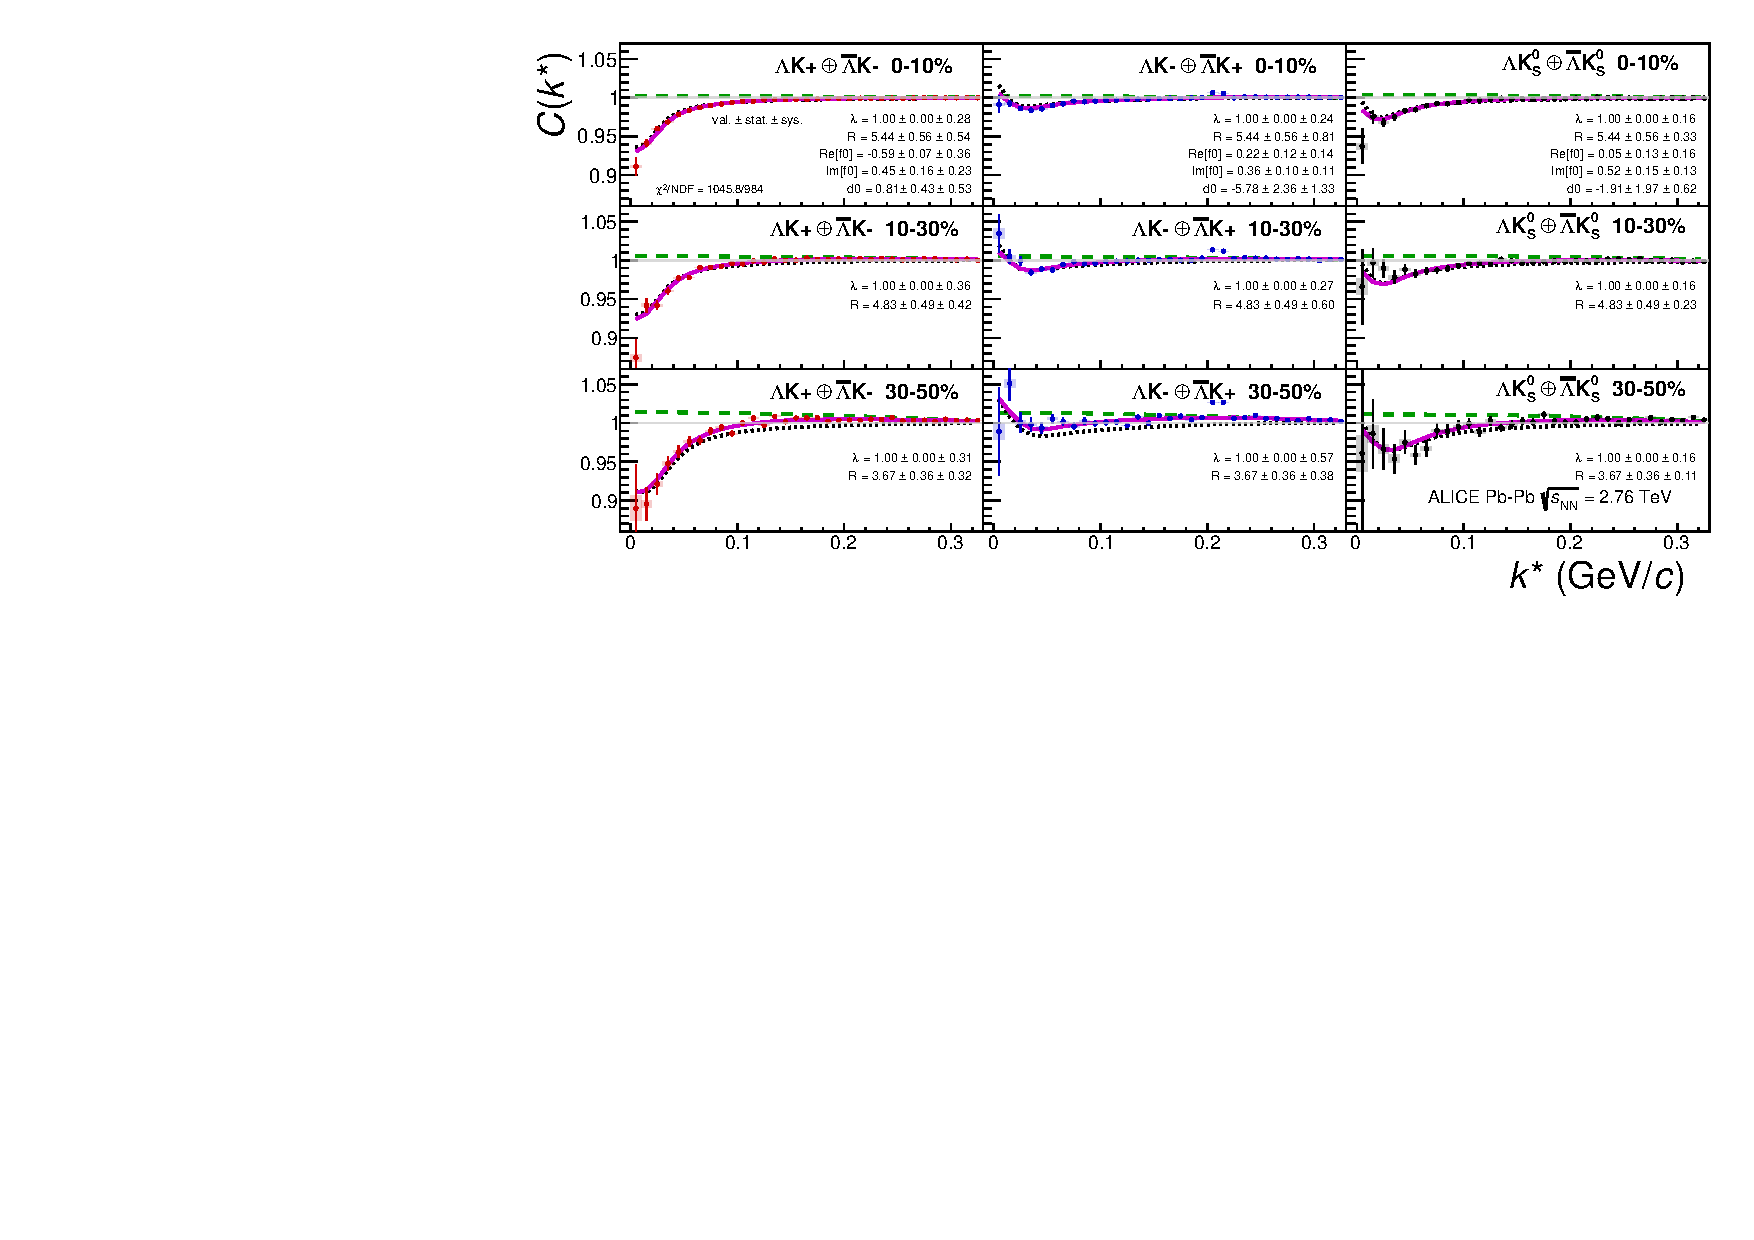
\includegraphics[width=\linewidth]{\ResultsDirBaseLamKs\SaveNameModLamKs/canKStarCfwFits_CombineConj_AllAn.pdf}
+  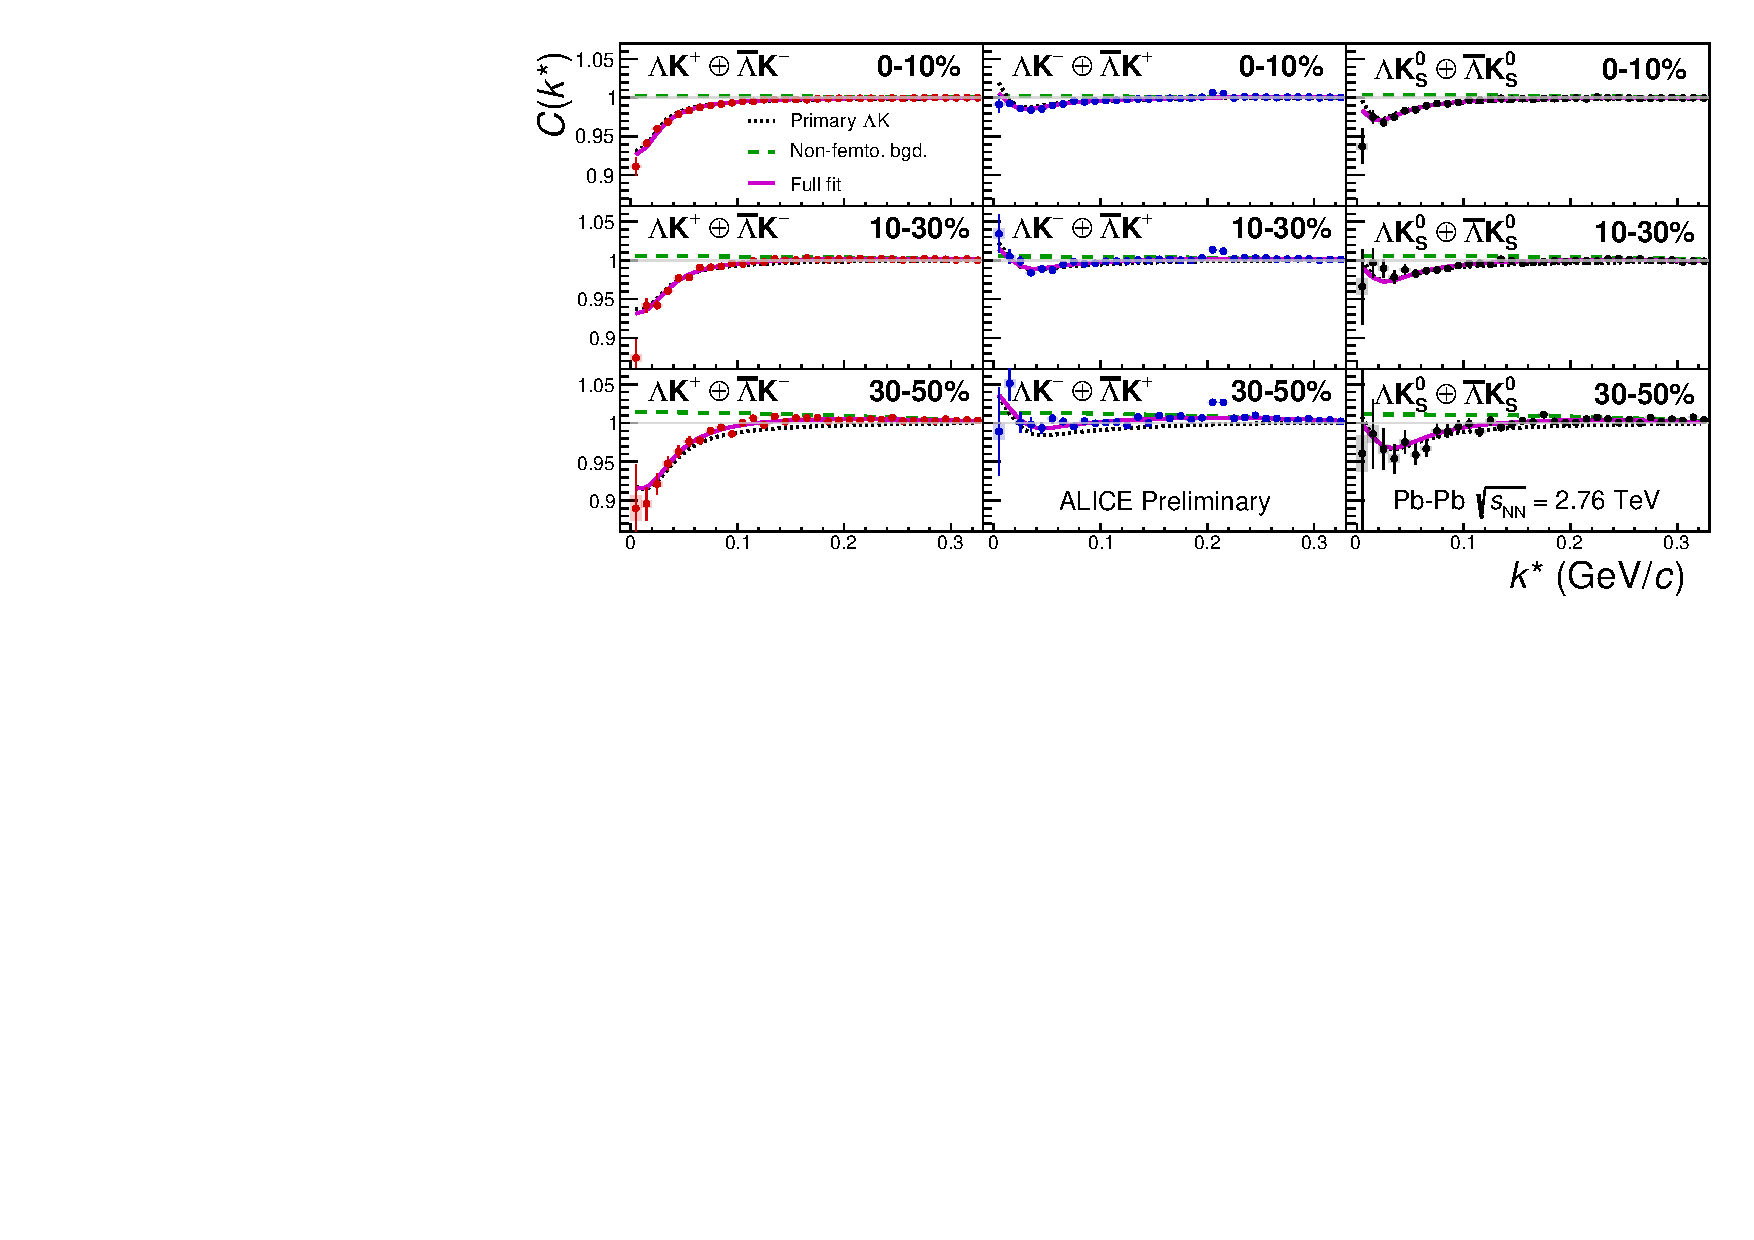
\includegraphics[width=\linewidth]{\ResultsDirBaseLamKch\SaveNameModLamKch/canKStarCfwFits_CombineConj_AllAn_LabelLines.pdf}
+  \caption[\LamK data with fits]
+  {
+  (Color online) Fit results for the \LamK data, with pair and conjugate combined.
+  The \LamKchP$\oplus$\ALamKchM data is shown in the left column, the \LamKchM$\oplus$\ALamKchP in the middle, and the \LamKs$\oplus$\ALamKs in the right. 
+  Rows differentiate the different centrality bins (0--10\% in the top, 10--30\% in the middle, and 30--50\% in the bottom).
+  See text for further details.
+ }
+  \label{fig:LamKFits_3Res}
+\end{figure}
 
 
 
@@ -1012,11 +1011,10 @@
   \label{fig:ScattParams_3Res}
 \end{figure}
 
-Figure \ref{fig:ScattParams_3Res} summarizes well the results of the present study.
-In the summary plot, the extracted scattering parameters are shown in the form of a $\Im f_{0}$ vs $\Re f_{0}$ plot, which includes the $d_{0}$ values to the right side.  
-Also shown are the $\lambda$ vs. radius parameters for all three studied centrality bins. 
-In addition to the results of this study, theoretical predictions made using chiral perturbation theory \cite{Liu:2006xja,Mai:2009ce} are shown.
-For all \LamK systems, positive imaginary parts of the scattering lengths, $\Im(f_{0})$, are extracted. 
+Figure \ref{fig:ScattParams_3Res} (left) summarizes the extracted \LamK scattering parameters, and includes theoretical predictions made using chiral perturbation theory \cite{Liu:2006xja,Mai:2009ce}.
+The predictions of Ref.\ \cite{Liu:2006xja} do not distinguish the K\Lam and K\ALam interactions and results are shown for two different parameter sets, whereas Ref.\ \cite{Mai:2009ce} offers unique K\Lam and $\overline{\mathrm{K}}$\Lam scattering parameters for a single parameter set. 
+In all cases, the predicted scattering parameters have both positive real and imaginary components, which is clearly inconsistent with the \LamKchP system.
+For all \LamK systems, positive imaginary parts of the scattering lengths, $\Im(f_{0})$, are extracted from the experimental data. 
 This is expected, as $\Im(f_{0})$ describes the inelastic scattering channels.
 More interestingly, the results show that the \LamKchP and \LamKchM systems differ in the sign of the real part, $\Re(f_{0})$, of their scattering lengths, with a negative value for \LamKchP and positive value for \LamKchM.
 The $\Re f_{0}$ extracted for the \LamKs system is positive, and within errors of that of the \LamKchM. 
@@ -1039,53 +1037,46 @@
   \label{fig:mTScalingOfRadii_3Res}
 \end{figure}
 
-A comparison of the extracted radii from this study to those of other systems measure by ALICE \cite{Adam:2015vja} is shown in Figure \ref{fig:mTScalingOfRadii_3Res}. 
-The figure shows extracted $R_{\mathrm{inv}}$ vs. \mt for several centralities and for several different systems.
+Figure \ref{fig:ScattParams_3Res} (right) presents the $\lambda$ vs. radius parameters for all three studied centrality bins. 
+Furthermore, a comparison of the extracted radii from this study to those of other systems measured by ALICE \cite{Adam:2015vja} is shown in Figure \ref{fig:mTScalingOfRadii_3Res}. 
+The figure shows extracted $R_{\mathrm{inv}}$ vs. \mt for several centralities and for several different pair systems.
 The \mt value used for the present \LamK results was taken as the average of the three systems\footnote[1]
 {
 For non-identical particle pairs, to be more directly analogous to the single particle \mt, the definition of the pair transverse mass used in this study is
 \begin{equation*}
 \begin{aligned}
- m_{\mathrm{T, pair}}^{2} &= \left( \frac{m_{\mathrm{inv}}}{2} \right)^{2} + \left( \frac{1}{2} |\textbf{\textit{p}}_{\mathrm{T,1}} + \textbf{\textit{p}}_{\mathrm{T,2}}| \right)^{2} \\
- &= (K^{0})^{2} - (K^{3})^{2} \\
- &\mathrm{where} ~~K^{\mu} \equiv \frac{1}{2} \left( p_{1}^{\mu} + p_{2}^{\mu} \right)
+ m_{\mathrm{T, pair}}^{2} &= \left( \frac{m_{\mathrm{inv}}}{2} \right)^{2} + \left( \frac{1}{2} |\textbf{\textit{p}}_{\mathrm{T,1}} + \textbf{\textit{p}}_{\mathrm{T,2}}| \right)^{2} = (K^{0})^{2} - (K^{3})^{2} \quad \mathrm{where} ~~K^{\mu} \equiv \frac{1}{2} \left( p_{1}^{\mu} + p_{2}^{\mu} \right)
 \end{aligned}
 \label{eqn:PairmTv1}
 \end{equation*}
 }.
 The radii are observed to increase for more central events, as expected from a simple geometric picture of the collisions.
-They also demonstrate a decreasing size with increasing \mt, as expected in the presence of collective radial flow \cite{Akkelin:1995gh}.
+They also demonstrate a decreasing size with increasing \mt in identical particle studies, as expected in the presence of collective radial flow \cite{Akkelin:1995gh}.
 It was found that \cite{Kisiel:2014upa}, even in the presence of good global \mt-scaling for the three-dimensional radii in the Longitudinally Co-Moving System (LCMS), a particle species dependence will exist for the $R_{\mathrm{inv}}$ measured in the Pair Rest Frame (PRF), due to trivial kinematic reasons.
 These kinematic effects, resulting from the transformation from LCMS to PRF, causes smaller masses to exhibit larger $R_{\mathrm{inv}}$ \cite{Adam:2015vja} (explaining, for instance, how the pion radii are systematically higher than kaon radii at the same approximate \mt).
 
-
 It is clear from the results in Fig.\ \ref{fig:mTScalingOfRadii_3Res} that the \LamK systems do not conform to the approximate \mt-scaling of the identical particle pair source sizes.
-At first thought, this may appear to be a troubling result; the approximate scaling is an observed consequence of the collective behavior of the soft (low-\pt) sector of the produced system.
-The \Lam and K particles certainly participate in the collective expansion of the QGP medium, but, importantly, they are non-identical particles, and all other systems in Fig.\ \ref{fig:mTScalingOfRadii_3Res} contain identical particles.
-In the case of identical particle femtoscopy, the pair source is comprised of two identical single particle sources, and the pair source size extracted is simply a factor $\sqrt{2}$ larger than those single particle sources.
-Thus, the identical particle pair source radii naturally follow the single particle source \mt-scaling in a simple manner.
-
-When dealing with non-identical particles, the pair emission source, which is measured by femtoscopy, is the superposition of two single-particle sources.
+When dealing with non-identical particles, the pair emission source is a superposition of two unique single-particle sources.
 The hydrodynamic nature of the medium produces the approximate \mt-scaling with respect to these single-particle sources, not the pair sources.
-More specifically, the hydrodynamic response of the system confines higher-\mt particles to smaller homogeneity regions, also pushes their average emission points further in the ``out" direction \cite{Retiere:2003kf}.
-Therefore, it is expected that the \Lam source is both smaller in size and further out in the fireball than that of the kaons.
-The combination of two unique sources separated in space-time, when probing correlations between non-identical particle pairs, can lead to extracted radii falling outside of the (identical particle femtoscopy) \mt-scaling trend.
-
-It is well established that non-identical particle femtoscopic studies are able to probe deeper than the second moments of the pair distribution functions accessed via identical particle studies.
-In addition to this, non-identical particle studies are able to measure the relative emission shifts, the first moments of the emission function \cite{Kisiel:2009eh}.
-For the study of \LamK pairs at mid-rapidity in Pb-Pb collisions, a separation of the single-particle sources in the out direction is expected.
-One elegant method for extracting information about the emission asymmetries is via a spherical decomposition of the correlation function.
+For identical particle studies, in which the pair source is comprised of two identical single particle sources, the femtoscopic radii naturally follow the \mt-scaling trend.
+The hydrodynamic response of the system not only confines higher-\mt particles to smaller homogeneity regions, but also pushes their average emission points further in the ``out" direction \cite{Retiere:2003kf}.
+Therefore, the \Lam and K sources differ both in size and space-time location, with the \Lam source both smaller in size and further out in the fireball than that of the kaons.
+These effects can inflate the radii extracted using the one-dimensional Lednick\'y model, which assumes a spherically symmetric source with no offsets (i.e. $R_{\mathrm{out}} = R_{\mathrm{side}} = R_{\mathrm{long}}$ and $\mu_{\mathrm{out}} = \mu_{\mathrm{side}} = \mu_{\mathrm{long}} = 0$).
+This effect is demonstrated in Appendix \ref{App:THERM} using the THERMINATOR 2 simulation.
+The largest violation of the \mt-scaling is observed for the 0--10\% centrality bin, in which one expects the largest emission asymmetry.
+In summary, the large extracted \LamK radii support the hydrodynamic nature of the system dictating the femtoscopic substructure.
+
+The experimental data support the difference in mean emission space-time coordinates of the \Lam and K sources, called an ``emission asymmetry".
+In addition to the second moments of the pair distribution functions, non-identical particle studies are sensitive to the relative emission shifts, i.e. the first moments of the emission function \cite{Kisiel:2009eh}.
+A separation of the single-particle sources in the out direction is expected for \LamK pairs at mid-rapidity in Pb-Pb collisions.
+The spherical harmonic decomposition of the correlation function offers an elegant method for extracting information about the emission asymmetries.
 With this method, one can draw a wealth of information from just a few components of the decomposition.
 Particularly, the $C_{00}$ component is similar to the 1D correlation functions typically studied, and probes the overall size of the source.
-The $\Re C_{11}$ component probes the asymmetry of the system in the out direction; a non-zero value reveals the asymmetry. 
-
-
+Of interest here, the $\Re C_{11}$ component probes the asymmetry of the system in the out direction; a non-zero value reveals the asymmetry. 
 Figure \ref{fig:LamKchP_ReC00C11_0010} shows the $C_{00}$ and $\Re C_{11}$ components from the spherical decomposition of the \LamKchP data in the 0--10\% centrality bin.
 The $\Re C_{11}$ component shows a clear deviation from zero, and the negative value signifies that the \Lam particles are, on average, emitted further out and/or earlier than the K mesons.
-This effect is supported by the results obtained from the THERMINATOR 2 model, shown in Fig.\ \ref{fig:LamKchP_StdThermSources}.
-The effect of a non-zero shift in the source will naturally lead to larger measured radii.
-This is intuitive, and also reaffirmed in the simulation with THERMINATOR 2 shown in App.\ \ref{App:THERM}.
-Larger effective radii are also found to result from inserting a Gaussian source with a non-zero shift into the Koonin-Pratt equation and numerically integrating.
+This conclusion is supported by the results obtained from the THERMINATOR 2 model, shown in Fig.\ \ref{fig:LamKchP_StdThermSources}.
+Furthermore, as previously stated, a non-zero shift in the source will induce larger extracted radii within the Lednick\'y model, as demonstrated with the THERMINATOR 2 simulatin in App.\ \ref{App:THERM}.
 
 \begin{figure}[h!]
   \centering
@@ -1099,21 +1090,18 @@
   \label{fig:LamKchP_ReC00C11_0010}
 \end{figure}
 
-It should be emphasized that the extracted \LamK source sizes do not indicate any sort of contradiction with the hydrodynamic nature of the system dictating the substructure of the femtoscopic radii.
-The results, rather, support this picture.
-As described above, the hydrodynamic response of the system confines the \Lam emission to smaller homogeneity regions located further out in the fireball, as compared to the kaons.
-Therefore, the single particle \Lam and K source sizes differ both in size and space-time location.
-When studying these pairs under the assumption of a spherically symmetric Gaussian source with no offset in the ``out" direction, this can lead to larger extracted radii, as demonstrated above with the THERMINATOR 2 simulation.
 
 \section{Summary}
 \label{sec:Summary}
 
-Results from a femtoscopic analysis of \LamK correlations in Pb-Pb collisions at $\sqrt{s_{\mathrm{NN}}}$ = 2.76 TeV with ALICE at the LHC have been presented.
+\subfile{\ResultsDirBaseLamKch\SaveNameModLamKch/Tables/ResultsTableTriple_Vert.tex}
+
+Results from a femtoscopic analysis of \LamK correlations in Pb-Pb collisions at $\sqrt{s_{\mathrm{NN}}}$ = 2.76 TeV with ALICE at the LHC have been presented, and are summarized in Table \ref{tab:FitResultsLamK_3Res}.
 The femtoscopic radii, $\lambda$ parameters, and scattering parameters were extracted from one-dimensional correlation functions in terms of the invariant momentum difference.
 The scattering parameters of \LamK pairs in all three charge combinations (\LamKchP, \LamKchM, and \LamKs) have been measured for the first time.
 Striking differences are observed in the \LamKchP, \LamKchM, and \LamKs correlation functions, which are reflected in the unique set of scattering parameters extracted for each.
 The extracted scattering parameters indicate that the strong force is repulsive in the \LamKchP interaction and attractive in the \LamKchM and \LamKs interactions.
-The physics underlying this phenomenon is currently not well understood, but this could be due to different quark-antiquark interactions between the pairs, or from different net strangeness for each system. 
+This effect could be due to different quark-antiquark interactions between the pairs, or from different net strangeness for each system. 
 The non-femtoscopic background is found to result almost entirely from collective effects, and is described quantitatively with unprecedented precision with the THERMINATOR 2 event generator.
 Finally, the \LamK systems exhibit source radii larger than expected from extrapolation from identical particle femtoscopic studies.
 This effect is interpreted as resulting from the separation in space-time of the single-particle \Lam and K source distributions.
@@ -1254,7 +1242,8 @@
 
 
 
-
+%%%%%%%%%%%%%%%%%%%%%%%%%%%%%%%%%%%%%%%%%%%%%%%%%%%%%%%%%%%%%%%%%%%%%%%%%%%%%%%%%%%%%%%%%%%%%%%%%%%%%%%%%%%%%
+\begin{comment}
 \section{Strong and Coulomb Fitter}
 \label{App:CoulombFitter}
 
@@ -1286,8 +1275,8 @@
 To build a fit function for a system including both strong and Coulomb interactions two related options were considered. 
 The first option was to numerically integrate Eq.\ \ref{eqn:KooninPrattEqn}.  
 The second option was to simulate a large sample of particle pairs, calculate the wave function describing the interaction, and average to obtain the integral in Eq.\ \ref{eqn:KooninPrattEqn}. 
-
-%\clearpage
+\end{comment}
+%%%%%%%%%%%%%%%%%%%%%%%%%%%%%%%%%%%%%%%%%%%%%%%%%%%%%%%%%%%%%%%%%%%%%%%%%%%%%%%%%%%%%%%%%%%%%%%%%%%%%%%%%%%%%
 
 
 %%%%%%%%%%%%%%%%%%%%%%%%%%%%%%%%%%%%%%%%%%%%%%%%%%%%%%%%%%%%%%%%%%%%%%%%%%%%%%%%%%%%%%%%%%%%%%%%%%%%%%%%%%%%%%%%%%%%%%%%%

